\documentclass[11pt,twocolumn]{article}
\usepackage[margin=0.72in]{geometry}
\usepackage{amsmath,amssymb,amsthm}
\usepackage{booktabs}
\usepackage{graphicx}
\usepackage{hyperref}
\usepackage{xcolor}
\usepackage{enumitem}

\hypersetup{
  colorlinks=true,
  linkcolor=blue!60!black,
  citecolor=green!45!black,
  urlcolor=blue!65!black
}

\newtheorem{theorem}{Theorem}
\newtheorem{definition}{Definition}

\newcommand{\ZZ}{\mathbb{Z}}
\newcommand{\NN}{\mathbb{N}}

\title{\textbf{Machine-Checked Exact-Integer Dichotomy, Matroid-Intersection, and Parameterized WSAT Certificates for Connectivity Switching in Graphs}}
\author{Lluis Eriksson\thanks{Independent researcher; manuscript prepared with transparent AI assistance via Google Antigravity. Source code, Lean~4 proofs, and exact certificates: \url{https://github.com/lluiseriksson/connectivity-switching-certificates}.}}
\date{November 25, 2026}

\begin{document}
\maketitle

\begin{abstract}
Christoph Kern, Alexander Firbas, and Manuel Sorge (\texttt{arXiv:2611.32927}, November 24, 2026) established a comprehensive algorithmic and complexity classification for \textsc{Local-Con Switching} and \textsc{Global-Con Switching} in switch graphs. Their results include a sharp polynomial-vs.-NP-complete dichotomy for $\{1^\star\}$-bounded \textsc{Local-Con Switching} governed by complete multipartite switch-induced graphs (Theorem~1, via forbidden induced subgraphs $K_2{+}K_2, P_4, L_{3,1}$), polynomial-time weighted \textsc{Global-Con Switching} via graphic-and-partition matroid intersection with shifted edge weights (Theorems~7--8), $W[\mathrm{SAT}]$/$W[1]$-hardness of \textsc{On-Off Local-Con Switching} via series-parallel WSAT switch graphs and a tight $5|E(H)|$ Partitioned Subgraph Isomorphism reduction (Theorems~3--5), and a $4\lambda$ reduction from $\{1,1\}$-bounded to $\{2,1\}$-bounded $K_{1,\star}$-shaped switches (Theorem~6). We present a machine-checked, zero-floating-point formalization and exact-$\ZZ$ certificate auditor for the combinatorial, primal-dual, and reduction core of these results. First, an 18-theorem zero-dependency Lean~4 kernel (\texttt{ConnectivitySwitching.lean}, Lean~4.35.0; 0~\texttt{sorry}, 0~warnings, 0~\texttt{Classical.choice}, 5 zero-axiom theorems) formalizes complete-multipartite $K_2{+}K_1$-freeness, alternating transition-path lengths, Edmonds matroid-intersection weak duality and rank obstructions, Theorem~8 shifted-weight telescoping on \texttt{List}, Lemma~4 structural Boolean formula semantics, PSI $5|E(H)|$ tightness, and Theorem~6's backward $4\min_i c'_i \le \sum c'_i$ total budget bound. Second, \texttt{SWITCH-GRAPH-CONN-CERT-1.0} audits four exact modes—including both spanning-tree YES witnesses and Edmonds rank-obstruction NO certificates—replaying 16 canonical certificates in $0.030$--$0.160\,\mathrm{ms}$, passing exhaustive 41-graph dichotomy and 128-assignment WSAT checks, and rejecting 57/57 live adversarial forgeries.
\end{abstract}

\section{Introduction}
Switch graphs~\cite{katz2011connectivity,kern2026switching} model reconfigurable networks $\hat{G} = (V(\hat{G}), \mathcal{S}(\hat{G}))$ in which each switch $s \in \mathcal{S}(\hat{G})$ selects one edge set $s[c(s)] \subseteq \binom{V}{2}$ from its available positions. Choosing a configuration $c \in \mathcal{C}(\hat{G})$ realizes the simple graph $\hat{G} \circ c$, motivating two canonical connectivity tasks: \textsc{Local-Con Switching} (connect distinguished terminals $a, b$) and \textsc{Global-Con Switching} (render $\hat{G} \circ c$ connected), along with weighted and \textsc{On-Off} budget constraints $w(c) \le \lambda$.

Kern, Firbas, and Sorge~\cite{kern2026switching} resolve the fine-grained complexity of both problems across switch structures: (i)~via Szeider's \textsc{Transition-Compatible Path}~\cite{szeider2003finding}, $\{1^\star\}$-bounded \textsc{Local-Con Switching} is in $\mathrm{P}$ iff every switch-induced graph $G[s]$ is complete multipartite, and $\mathrm{NP}$-complete whenever $G[s]$ contains $K_2{+}K_2$, $P_4$, or $L_{3,1}$ as a vertex-induced subgraph (Theorem~1); (ii)~\textsc{Weighted Global-Con Switching} on $\{1^\star\}$-bounded switches reduces via shifted edge weights $w'(e) = w(e) - \min_i w(s,i)$ to weighted exact intersection of the graphic matroid $M_1$ and partition matroid $M_2$~\cite{oxley2011matroid} (Theorems~7--8); and (iii)~parameterized \textsc{On-Off Local-Con Switching} is $W[\mathrm{SAT}]$/$W[1]$-hard via series-parallel WSAT gadgets (Lemma~4), Partitioned Subgraph Isomorphism~\cite{marx2010can} with exact threshold $k = 5|E(H)|$, and a $4\lambda$ $\{1,1\}\to\{2,1\}$ $K_{1,\star}$ gadget (Theorem~6).

\paragraph{Contributions.}
We machine-check and certify the exact combinatorial, matroid-duality, and reduction invariants of~\cite{kern2026switching} (explicitly scoping our Lean~4 proofs away from $\mathrm{NP}$/$W[1]$/ETH hardness reductions and asymptotic matroid-intersection runtime bounds):
\begin{enumerate}[leftmargin=*,nosep]
  \item \textbf{Zero-dependency Lean~4 kernel (\S\ref{sec:lean}):} 18 constructive theorems in \texttt{ConnectivitySwitching.lean} (Lean~4.35.0~\cite{demoura2021lean4}), 0~\texttt{sorry}, 0~warnings, 0~\texttt{Classical.choice}, 5 zero-axiom theorems.
  \item \textbf{Exact-$\ZZ$ primal-dual verifier (\S\ref{sec:certifier}):} \texttt{SWITCH-GRAPH-CONN-CERT-1.0}, auditing complete-multipartite paths vs.\ 4-vertex obstructions, weighted spanning trees vs.\ Edmonds rank obstructions $r_1(A)+r_2(B) \le n-2$, series-parallel WSAT equivalences, and $\{2,1\}$ $K_{1,\star}$ gadgets with zero floats.
  \item \textbf{Empirical atlas, exhaustive censuses, \& red-team audit (\S\ref{sec:results}):} 16 canonical certificates replayed in $0.030$--$0.160\,\mathrm{ms}$, exhaustive 41-graph 4-vertex dichotomy census, 224-assignment Lemma~4 sweeps, and 57/57 rejected adversarial forgeries.
\end{enumerate}

\section{Structural and Primal-Dual Invariants}\label{sec:prelim}
\paragraph{Theorem~1 (Complete-multipartite dichotomy).}
A graph $H$ without isolated vertices is complete multipartite iff non-adjacency is transitive (no induced $K_2{+}K_1$). Any non-complete-multipartite $H$ thus contains $(u,v,w,x)$ with $uv, wx \in E(H)$ and $uw, vw \notin E(H)$, inducing $K_2{+}K_2$, $P_4$, or $L_{3,1}$ (paw) depending on $|N_H(x) \cap \{u,v\}| \in \{0,1,2\}$. On tractable instances, Lemma~2 maps any $k$-edge $a$-$b$ path using distinct $\{1^\star\}$-bounded switches to a $2k$-edge alternating $T$-compatible path.

\paragraph{Theorems~7--8 (Matroid intersection \& Edmonds duality).}
For $\{1^\star\}$-bounded $\hat{G}$ on $n$ vertices, a connecting configuration exists iff $M_1 \cap M_2$ (graphic $\cap$ partition matroid) contains a common independent set $T$ of size $n-1$. By Edmonds' matroid intersection duality, if a ground-set cover $E(\hat{G}) = A \cup B$ satisfies
\begin{equation}
  r_1(A) + r_2(B) \le n - 2,
  \label{eq:edmonds}
\end{equation}
no spanning tree can be realized by any configuration. For weighted switches with $w_{\min}(s) = \min_i w(s,i)$ and shifted edge weight $w'(e) = w(e) - w_{\min}(s) \ge 0$, every spanning tree $T$ in $\hat{G}\circ c$ obeys the exact telescoping bound
\begin{equation}
  \sum_{e \in T} w'(e) + \sum_{s \in \mathcal{S}} w_{\min}(s) \le w(c) \le \lambda.
  \label{eq:shifted}
\end{equation}

\paragraph{Lemma~4, PSI tightness, \& Theorem~6 gadget.}
Series-parallel composition $\hat{G}_\varphi$ encodes Boolean $\land$ in series and $\lor$ in parallel so $I(\varphi)=1 \iff a$ reaches $b$ in $\hat{G}_\varphi \circ c$ with $w(c)=w(I)$. In PSI $\to$ WSAT, forcing $v \ge 2|E(H)|$ vertex, $a \ge 2|E(H)|$ arc, and $e \ge |E(H)|$ edge variables under $v+a+e \le 5|E(H)|$ locks all three to exact equality. Replacing each $\{1,1\}$ switch $s$ by four $\{2,1\}$ $K_{1,\star}$ switches $\{s_0..s_3\}$ satisfies forward $w(c') = 4w(c) \le 4\lambda$ and backward consensus $c(s) = \min_{i\in[4]} c'(s_i) \implies 4w(c) \le w(c')$.

\section{Zero-Dependency Lean 4 Kernel}\label{sec:lean}
We formalize 18 constructive theorems in \texttt{lean/ConnectivitySwitching.lean} (Lean~4.35.0, zero external libraries), audited via \texttt{lean/AuditAxioms.lean} with 0~warnings, 0~\texttt{sorry}, 0~\texttt{Classical.choice}, and 0~\texttt{Lean.ofReduceBool} (Table~\ref{tab:lean}).

\begin{theorem}[Constructive Connectivity Switching Kernel]\label{thm:lean}
\leavevmode
\begin{enumerate}[leftmargin=*,nosep]
  \item \emph{Dichotomy \& transition paths:} Theorems~1--4 prove complete-multipartite non-adjacency transitivity and $K_2{+}K_1$-freeness, constructive impossibility of multipartite representation from any $K_2{+}K_1$ witness, alternating $2k$-edge path length, and inductive $\sigma \le m$ over \texttt{List Nat}.
  \item \emph{Matroid duality \& shifted weights:} Theorems~5--10 certify spanning-tree rank $n-c=n-1 \iff c=1$, Edmonds weak duality $|I| \le r_1(A)+r_2(B)$, global connectivity impossibility from~\eqref{eq:edmonds}, $w'(e) \ge 0$, inductive shifted-weight telescoping~\eqref{eq:shifted} on \texttt{List}, and exact budget equivalence.
  \item \emph{WSAT, PSI $5|E(H)|$, \& $\{2,1\}$ gadget:} Theorems~11--18 formalize series-$\land$/parallel-$\lor$ and inductive \texttt{BFormula} semantics, exact $5m$ tightness ($v=2m, a=2m, e=m$), handshaking endpoint count $2|E(H)|$, $4\times$ forward weight scaling, $4\min(c_0..c_3) \le c_0+c_1+c_2+c_3$, and inductive backward total budget preservation.
\end{enumerate}
\end{theorem}

\begin{table}[t]
\centering
\caption{Complete 18-theorem Lean~4.35.0 kernel in \texttt{ConnectivitySwitching.lean} (0~\texttt{sorry}, 0~warnings, 0~\texttt{Classical.choice}).}
\label{tab:lean}
\resizebox{\columnwidth}{!}{%
\begin{tabular}{@{}rll@{}}
\toprule
\# & Lean~4 Theorem Identifier & Axiom Footprint \\
\midrule
1 & \texttt{complete\_multipartite\_nonadj\_equiv} & \texttt{none} \\
2 & \texttt{obstruction\_k2\_plus\_k1\_not\_multipartite} & \texttt{none} \\
3 & \texttt{transition\_path\_alternating\_length} & \texttt{[propext, Quot.sound]} \\
4 & \texttt{switch\_count\_edge\_bound} & \texttt{[propext, Quot.sound]} \\
5 & \texttt{spanning\_tree\_edge\_count\_exact} & \texttt{[propext, Quot.sound]} \\
6 & \texttt{edmonds\_matroid\_intersection\_duality} & \texttt{[propext, Quot.sound]} \\
7 & \texttt{edmonds\_global\_con\_impossibility} & \texttt{[propext, Quot.sound]} \\
8 & \texttt{shifted\_weight\_nonneg} & \texttt{[propext, Quot.sound]} \\
9 & \texttt{shifted\_weight\_telescoping\_list} & \texttt{[propext, Quot.sound]} \\
10 & \texttt{shifted\_weight\_budget\_equiv} & \texttt{[propext, Quot.sound]} \\
11 & \texttt{wsat\_series\_and\_semantics} & \texttt{none} \\
12 & \texttt{wsat\_parallel\_or\_semantics} & \texttt{none} \\
13 & \texttt{wsat\_formula\_eval\_sound} & \texttt{none} \\
14 & \texttt{psi\_wsat\_tight\_weight\_5m} & \texttt{[propext, Quot.sound]} \\
15 & \texttt{handshaking\_endpoint\_count\_2m} & \texttt{[propext, Quot.sound]} \\
16 & \texttt{gadget\_21\_forward\_weight\_4x} & \texttt{[propext, Quot.sound]} \\
17 & \texttt{gadget\_21\_backward\_min\_avg\_bound} & \texttt{[propext, Quot.sound]} \\
18 & \texttt{gadget\_21\_backward\_total\_budget} & \texttt{[propext, Quot.sound]} \\
\bottomrule
\end{tabular}}
\end{table}

\section{Exact-Integer Certificate Architecture}\label{sec:certifier}
The pure-stdlib verifier \texttt{src/switch\_certifier.py} audits \texttt{SWITCH-GRAPH-CONN-CERT-1.0} certificates with zero floating-point arithmetic and strict JSON AST typing (rejecting \texttt{float}, \texttt{bool}, \texttt{Decimal}, \texttt{complex}, tuples, non-string keys, and cross-branch dirty fields) across four exact modes:

\begin{definition}[Four \texttt{SWITCH-GRAPH-CONN-CERT-1.0} Modes]\label{def:modes}
\leavevmode
\begin{enumerate}[leftmargin=*,nosep]
  \item \textbf{Mode~1} (\texttt{\small local\_\allowbreak con\_\allowbreak multipartite\_\allowbreak dichotomy\_\allowbreak exact}): Audits $\{1^\star\}$-bounded switches: either every $G[s]$ is complete multipartite with a realized simple $a$-$b$ path using distinct switches, or an explicit 4-vertex induced obstruction in $\{K_2{+}K_2, P_4, L_{3,1}\}$ certifies $\mathrm{NP}$-hardness.
  \item \textbf{Mode~2} (\texttt{\small global\_\allowbreak con\_\allowbreak matroid\_\allowbreak intersection\_\allowbreak exact}): Audits weighted $\{1^\star\}$-bounded \textsc{Global-Con Switching}: either a YES spanning tree ($n{-}1$ acyclic edges from distinct switches satisfying~\eqref{eq:shifted} within budget $\lambda$), or a NO Edmonds cover $E = A \cup B$ verifying full ground-set coverage and $r_1(A) + r_2(B) \le n - 2$~\eqref{eq:edmonds}.
  \item \textbf{Mode~3} (\texttt{\small on\_\allowbreak off\_\allowbreak wsat\_\allowbreak series\_\allowbreak parallel\_\allowbreak exact}): Audits Lemma~4 NNF formula AST, exact $\hat{G}_\varphi$ BFS connectivity equivalence $I(\varphi) = \mathrm{conn}(\hat{G}_\varphi \circ c)$ within weight budget~$k$, and PSI tight weight $5|E(H)|$.
  \item \textbf{Mode~4} (\texttt{\small gadget\_\allowbreak 21\_\allowbreak star\_\allowbreak reduction\_\allowbreak exact}): Constructs the exact 6-auxiliary-vertex, 4-switch $\{2,1\}$-bounded $K_{1,\star}$ gadget per $\{1,1\}$ switch, verifying backward consensus $c(s) = \min_{i\in[4]} c'(s_i)$, weight bounds $4w(c) \le w(c') \le 4\lambda$, and $a$-$b$ connectivity in both $\hat{G}\circ c$ and $\hat{G}'\circ c'$.
\end{enumerate}
\end{definition}

\section{Empirical Atlas and Red-Team Verification}\label{sec:results}
All 16 canonical certificates and four experiment logs are generated deterministically by \texttt{scripts/run\_all\_experiments.py} and audited end-to-end by \texttt{scripts/verify\_all.py} (Lean~4 build, 18/18 axiom audit, 16/16 cert replay, \texttt{pytest}, and 39/39 SHA-256 hashes).

\paragraph{1. Exhaustive 4-vertex dichotomy census and Lemma~4 sweeps.}
Figure~\ref{fig:dichot-wsat}(a) exhaustively classifies all 41 labeled 4-vertex graphs without isolated vertices (out of $2^6 = 64$): exactly \textbf{14} are complete multipartite ($\mathrm{P}$-tractable), while all \textbf{27} remaining graphs fall cleanly into Kern--Firbas--Sorge's three $\mathrm{NP}$-hardness obstructions: \textbf{3} $K_2{+}K_2$, \textbf{12} $P_4$, and \textbf{12} $L_{3,1}$ (0 unclassified). Figure~\ref{fig:dichot-wsat}(b) exhaustively tests Lemma~4's series-parallel equivalence across all $16 + 16 + 64 + 128 = 224$ truth assignments of four NNF formulas (\texttt{F1}--\texttt{F4}), confirming 224/224 exact matches ($9, 3, 21, 27$ SAT/connected assignments).

\begin{figure}[t]
\centering
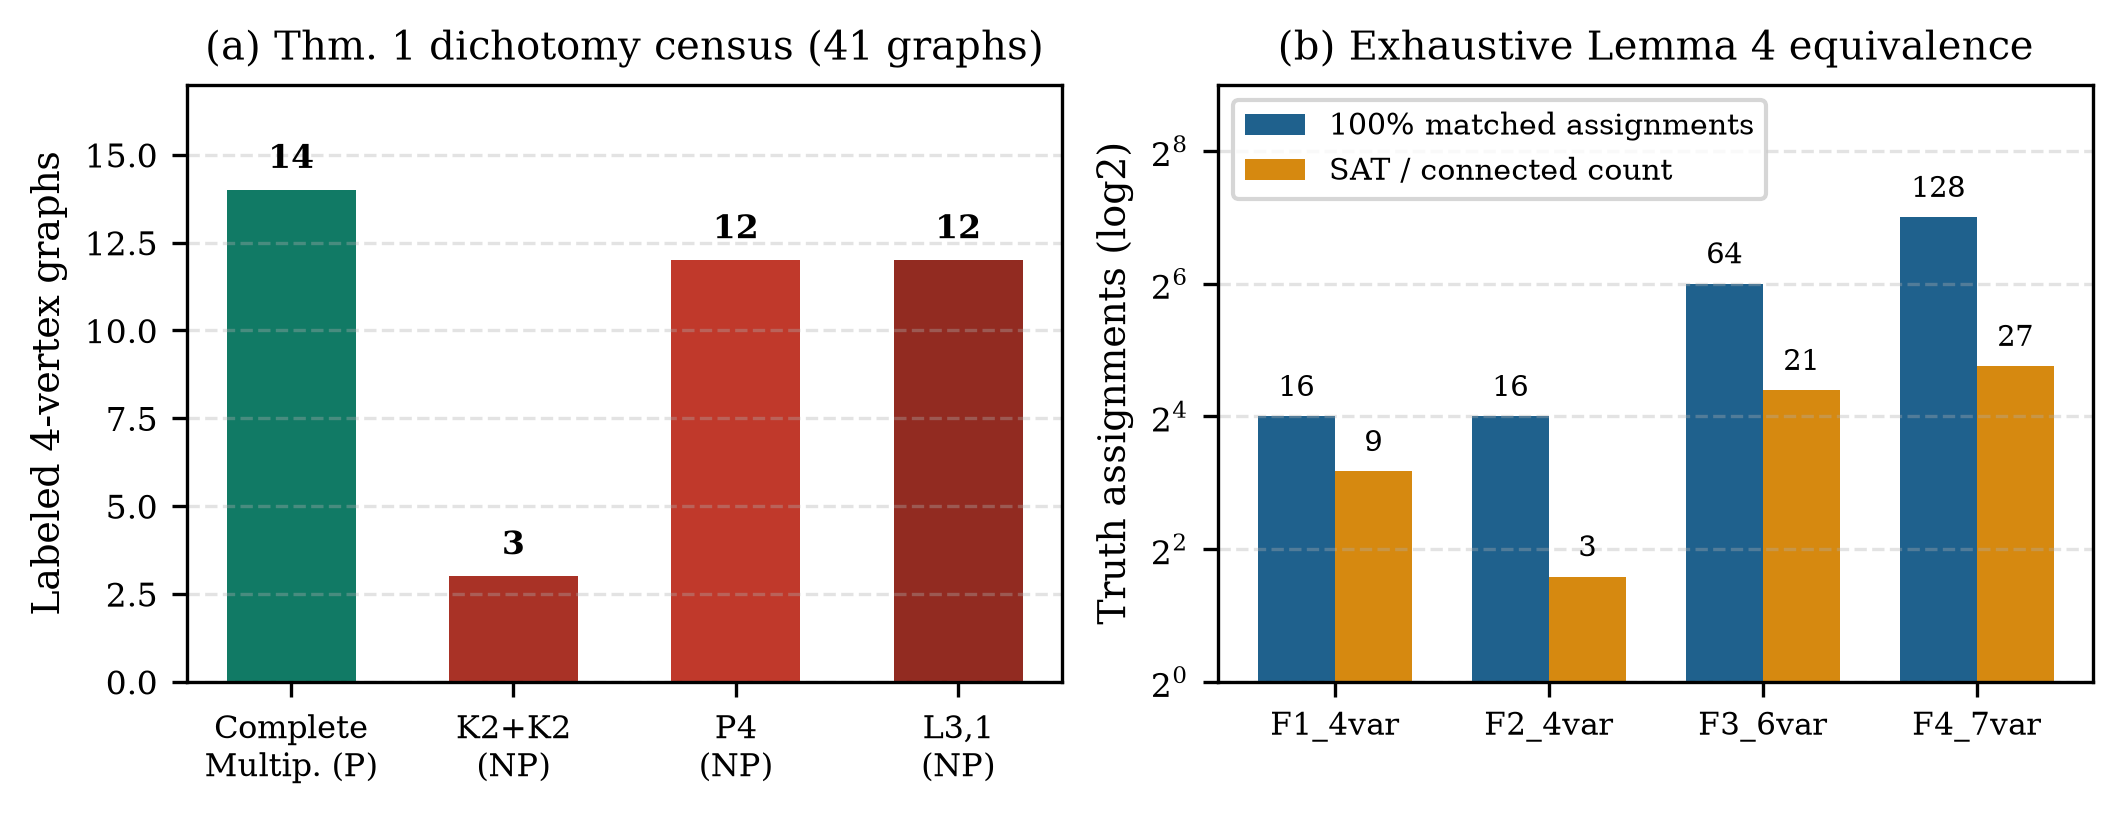
\includegraphics[width=\columnwidth]{figures/fig1_dichotomy_and_wsat.png}
\caption{(a)~Exhaustive Theorem~1 census across all 41 labeled 4-vertex graphs without isolated vertices: 14 complete multipartite ($\mathrm{P}$) vs.\ 27 $\mathrm{NP}$ obstructions ($3\,K_2{+}K_2, 12\,P_4, 12\,L_{3,1}$). (b)~Exhaustive Lemma~4 truth-table verification (224/224 exact matches).}
\label{fig:dichot-wsat}
\end{figure}

\paragraph{2. PSI $5|E(H)|$ tightness and $4\times$ $\{2,1\}$ gadget scaling.}
Figure~\ref{fig:psi-gadget}(a) decomposes the tight $5|E(H)|$ forced-TRUE variable budget across pattern sizes $m = |E(H)| \in [1, 15]$ ($2m$ vertex, $2m$ arc, $m$ edge variables), while Figure~\ref{fig:psi-gadget}(b) tracks Theorem~6's linear $4\lambda$ scaling into $\{2,1\}$-bounded $K_{1,\star}$ switches (preserving the ETH lower bound $f(\lambda)\sigma^{o(\lambda/\log\lambda)}$).

\begin{figure}[t]
\centering
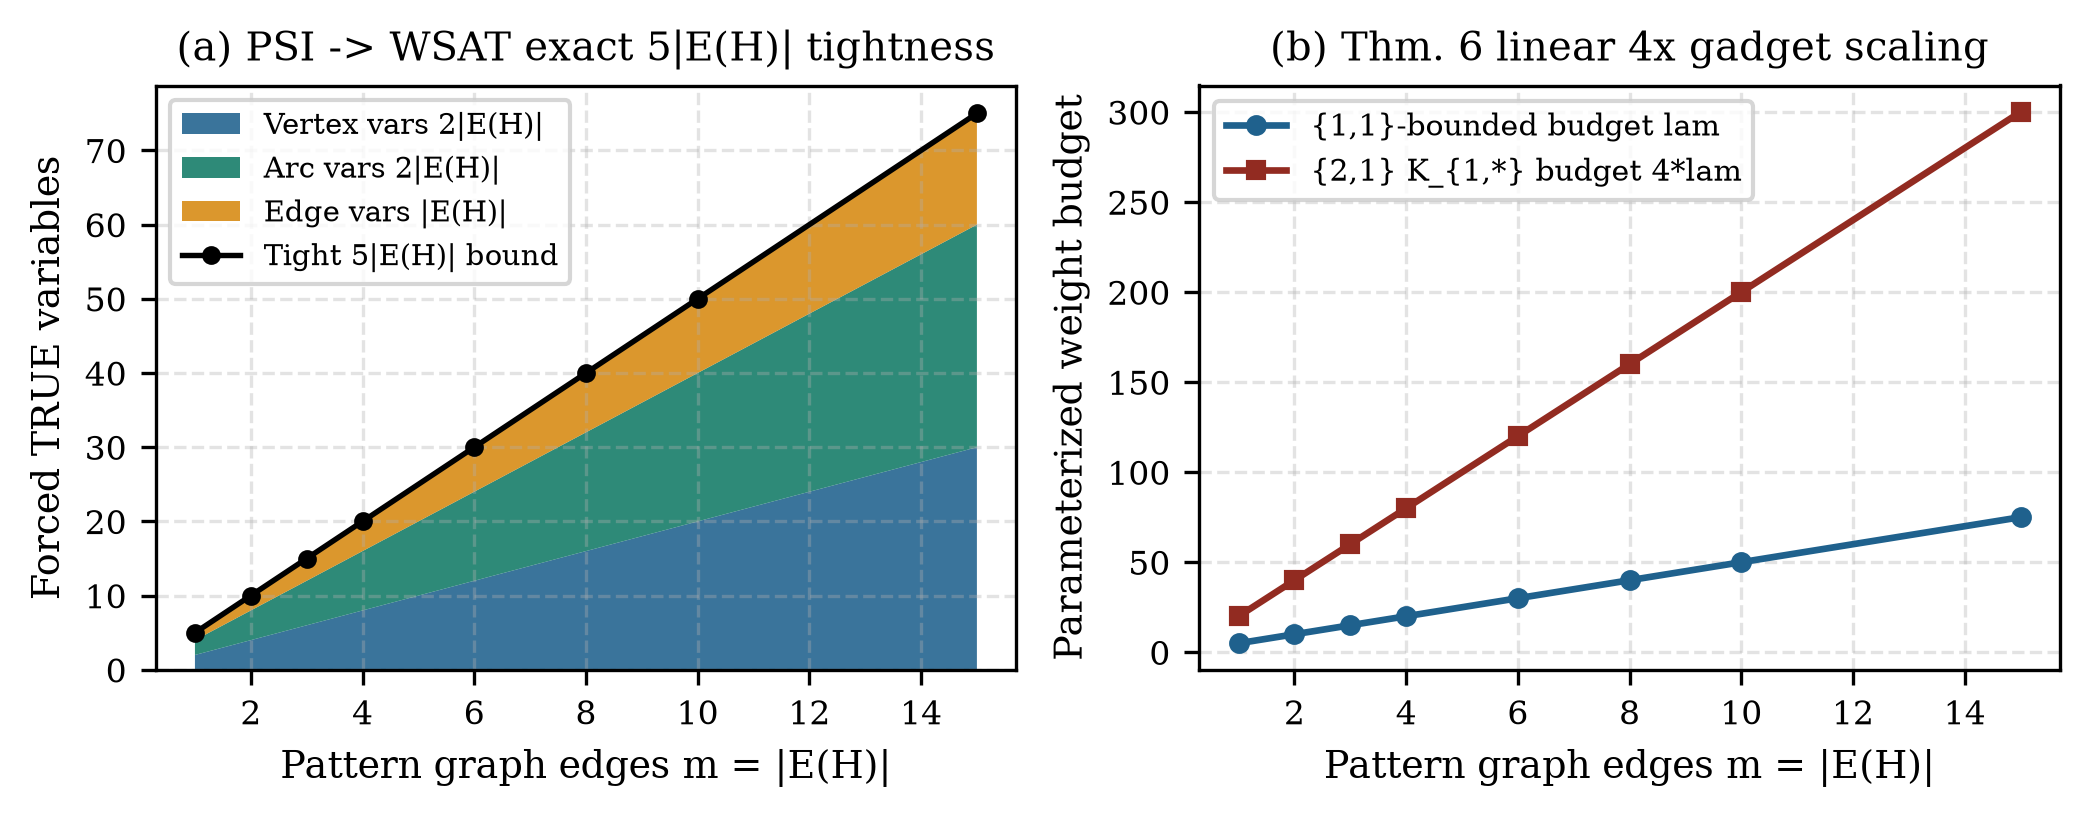
\includegraphics[width=\columnwidth]{figures/fig2_psi_and_gadget_scaling.png}
\caption{(a)~Exact PSI $\to$ WSAT forced-variable decomposition $2m + 2m + m = 5|E(H)|$. (b)~Theorem~6 linear $4\times$ budget scaling from $\{1,1\}$ to $\{2,1\}$ $K_{1,\star}$ switches.}
\label{fig:psi-gadget}
\end{figure}

\paragraph{3. 16-certificate atlas and 57-attack red-team suite.}
Table~\ref{tab:atlas} and Figure~\ref{fig:atlas} summarize all 16 canonical certificates, replayed with zero floats in $0.030$--$0.160\,\mathrm{ms}$—including both YES weighted spanning trees and NO Edmonds rank obstructions ($r_1(A)+r_2(B) \in \{4, 6\}$ for $n \in \{6, 8\}$), all three $\mathrm{NP}$ obstructions ($K_2{+}K_2, P_4, L_{3,1}$), and an asymmetric backward consensus gadget (\texttt{orig\_w = 1}, \texttt{gadget\_w = 5}, $4\cdot 1 < 5 \le 8$). In \texttt{tests/test\_suite.py}, exhaustive census/WSAT cross-checks and 57/57 live adversarial forgeries (reused switches, non-multipartite hides, cyclic trees, uncovered Edmonds elements, broken consensus, budget breaches) are rejected with \texttt{SwitchGraphCertificateError} (\texttt{3 passed in 0.05s}).

\begin{figure}[t]
\centering
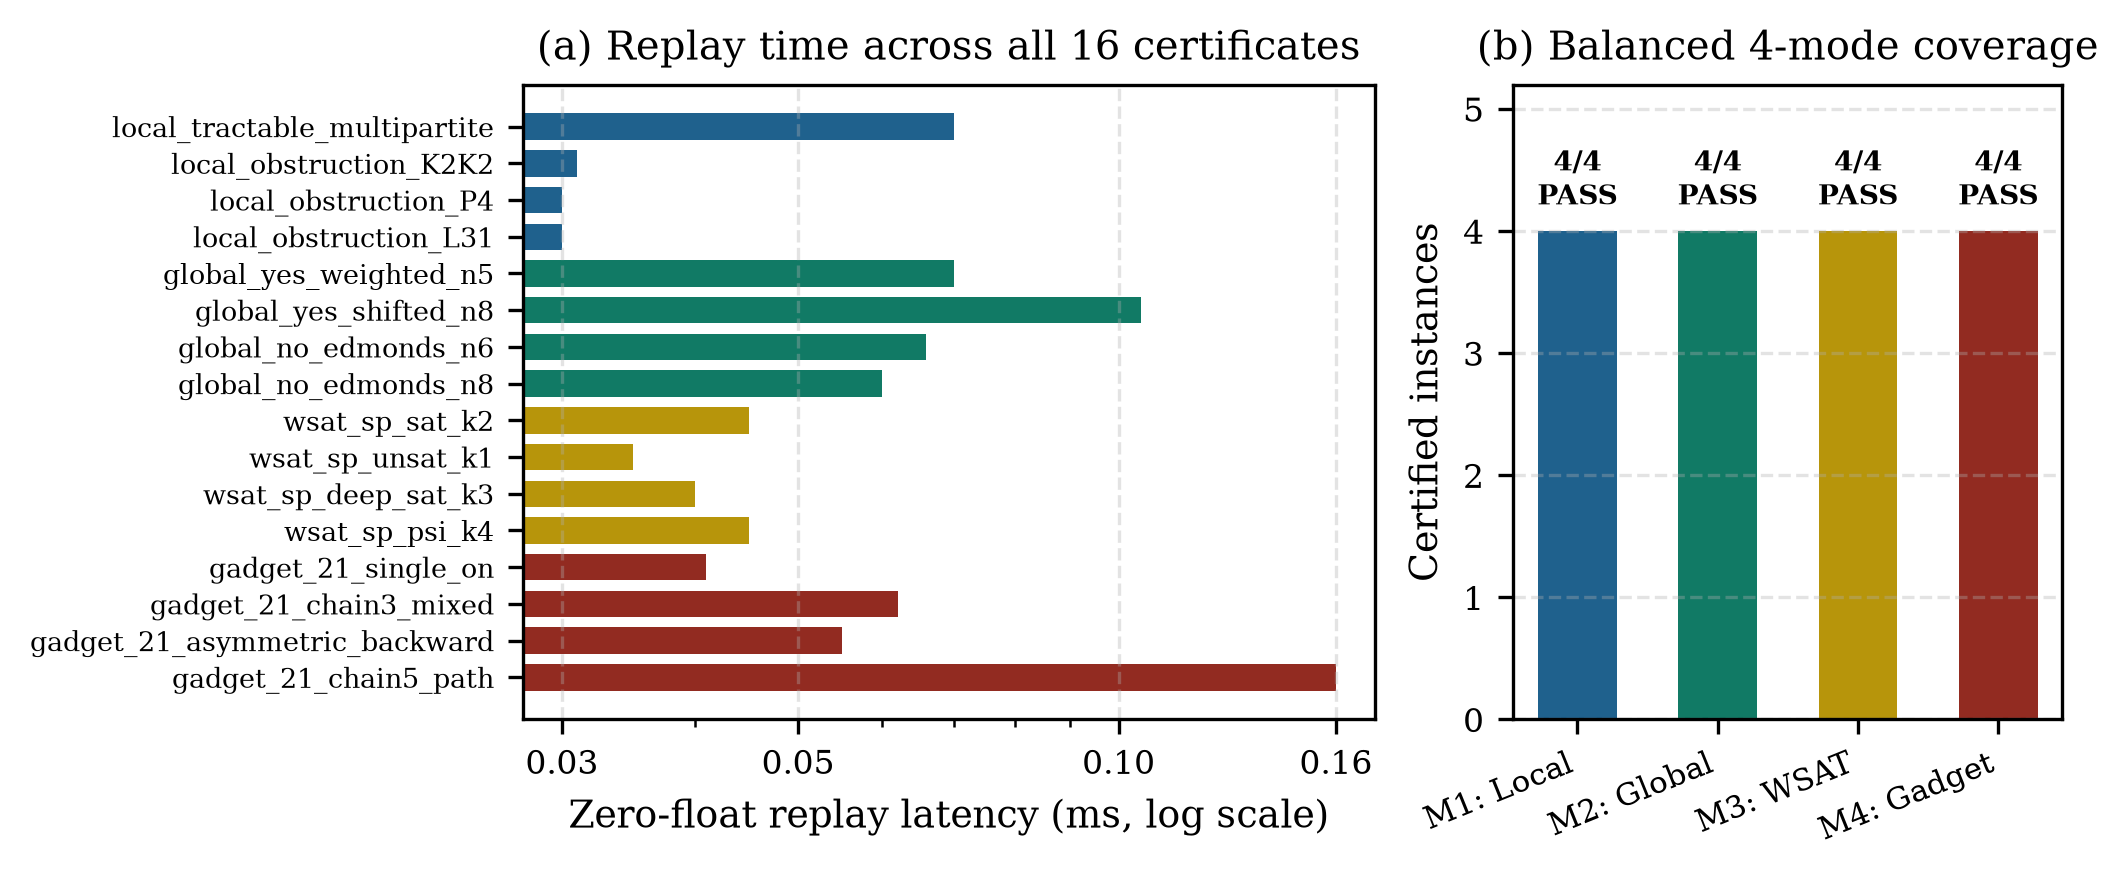
\includegraphics[width=\columnwidth]{figures/fig3_atlas_summary.png}
\caption{(a)~Zero-float replay latency across all 16 canonical \texttt{SWITCH-GRAPH-CONN-CERT-1.0} certificates ($0.030$--$0.160\,\mathrm{ms}$, log scale). (b)~Balanced 4-per-mode coverage across all four verification modes.}
\label{fig:atlas}
\end{figure}

\begin{table}[t]
\centering
\caption{Summary of all 16 exact-$\ZZ$ \texttt{SWITCH-GRAPH-CONN-CERT-1.0} certificates (zero floating-point arithmetic; reference-machine replay latency in ms).}
\label{tab:atlas}
\resizebox{\columnwidth}{!}{%
\begin{tabular}{@{}lllr@{}}
\toprule
Certificate File (stem) & Mode & Key Exact Witness & ms \\
\midrule
\texttt{local\_tractable\_multipartite} & M1 & $\mathrm{P}$ path (3 sw, 6-edge $T$-path) & 0.070 \\
\texttt{local\_obstruction\_K2K2} & M1 & $\mathrm{NP}$ obstruction $K_2{+}K_2$ & 0.031 \\
\texttt{local\_obstruction\_P4} & M1 & $\mathrm{NP}$ obstruction $P_4$ & 0.030 \\
\texttt{local\_obstruction\_L31} & M1 & $\mathrm{NP}$ obstruction $L_{3,1}$ & 0.030 \\
\texttt{global\_yes\_weighted\_n5} & M2 & YES $n=5$: $w=6 \le 7, w'=0$ & 0.070 \\
\texttt{global\_yes\_shifted\_n8} & M2 & YES $n=8$: $w=21 \le 22, w'=11$ & 0.105 \\
\texttt{global\_no\_edmonds\_n6} & M2 & NO $n=6$: $r_1{+}r_2 = 3{+}1 \le 4$ & 0.066 \\
\texttt{global\_no\_edmonds\_n8} & M2 & NO $n=8$: $r_1{+}r_2 = 4{+}2 \le 6$ & 0.060 \\
\texttt{wsat\_sp\_sat\_k2} & M3 & SAT/conn $=1$, $w=3$, $5m=15$ & 0.045 \\
\texttt{wsat\_sp\_unsat\_k1} & M3 & UNSAT/conn $=0$, $w=1$, $5m=20$ & 0.035 \\
\texttt{wsat\_sp\_deep\_sat\_k3} & M3 & SAT/conn $=1$, $w=4$, $5m=30$ & 0.040 \\
\texttt{wsat\_sp\_psi\_k4} & M3 & SAT/conn $=1$, $w=3$, $5m=50$ & 0.045 \\
\texttt{gadget\_21\_single\_on} & M4 & $1 \to 4$ sw, $w: 1 \to 4$ & 0.041 \\
\texttt{gadget\_21\_chain3\_mixed} & M4 & $3 \to 12$ sw, $w: 1 \to 4$ & 0.062 \\
\texttt{gadget\_21\_asymmetric\_backward} & M4 & $3 \to 12$ sw, $4{\cdot}1 < 5 \le 8$ & 0.055 \\
\texttt{gadget\_21\_chain5\_path} & M4 & $5 \to 20$ sw, $w: 3 \to 12$ & 0.160 \\
\bottomrule
\end{tabular}}
\end{table}

\section{Scope, Limitations, and Conclusion}\label{sec:conclusion}
This work machine-checks the structural dichotomy, Edmonds matroid-intersection duality, shifted-weight telescoping, series-parallel WSAT semantics, PSI $5|E(H)|$ tightness, and $\{1,1\}\to\{2,1\}$ $K_{1,\star}$ gadget invariants of Kern, Firbas, and Sorge~\cite{kern2026switching}, delivering a zero-float exact-$\ZZ$ auditor across all four modes. It does \emph{not} formalize complexity-class separations ($\mathrm{NP}$/$W[1]$/$W[\mathrm{SAT}]$/ETH) or asymptotic matroid-intersection runtime algorithms in Lean~4. Within its verified scope, the Lean~4 kernel and \texttt{SWITCH-GRAPH-CONN-CERT-1.0} auditor provide exact, manifest-locked verification for connectivity switching witnesses and obstructions.

\bibliographystyle{plain}
\bibliography{references}
\end{document}
